\documentclass[12pt]{article}

% Preamble: use same packages as main file
% Packages
\usepackage{amssymb,amsmath,amsthm,bbm}
\usepackage{verbatim,float,url,dsfont}
\usepackage{graphicx,subcaption,psfrag}
\usepackage{algorithm,algorithmic}
\usepackage{mathtools,enumitem}
\usepackage{multirow}
\usepackage{ragged2e}
\usepackage{xr-hyper}
\usepackage{array}

\usepackage[colorlinks=true,citecolor=blue,urlcolor=blue,linkcolor=blue]{hyperref}
\usepackage[margin=1in]{geometry}
\usepackage[round]{natbib}

\usepackage[utf8]{inputenc} % allow utf-8 input
\usepackage[T1]{fontenc}    % use 8-bit T1 fonts
\usepackage{booktabs}       % professional-quality tables
\usepackage{nicefrac}         % compact symbols for 1/2, etc.
\usepackage{microtype}      % microtypography

\ifdefined\TimesFont 
\usepackage{times} % use times font
\fi

\ifdefined\ParSkip 
\usepackage{parskip} % use par skip
\fi

% Theorems and such
\newtheorem{theorem}{Theorem}
\newtheorem{lemma}{Lemma}
\newtheorem{corollary}{Corollary}
\newtheorem{proposition}{Proposition}
\theoremstyle{definition}
\newtheorem{remark}{Remark}
\newtheorem{definition}{Definition}

% Assumption
\newtheorem*{assumption*}{\assumptionnumber}
\providecommand{\assumptionnumber}{}
\makeatletter
\newenvironment{assumption}[2]{
  \renewcommand{\assumptionnumber}{Assumption #1#2}
  \begin{assumption*}
  \protected@edef\@currentlabel{#1#2}}
{\end{assumption*}}
\makeatother

% Widebar
\makeatletter
\newcommand*\rel@kern[1]{\kern#1\dimexpr\macc@kerna}
\newcommand*\widebar[1]{%
  \begingroup
  \def\mathaccent##1##2{%
    \rel@kern{0.8}%
    \overline{\rel@kern{-0.8}\macc@nucleus\rel@kern{0.2}}%
    \rel@kern{-0.2}%
  }%
  \macc@depth\@ne
  \let\math@bgroup\@empty \let\math@egroup\macc@set@skewchar
  \mathsurround\z@ \frozen@everymath{\mathgroup\macc@group\relax}%
  \macc@set@skewchar\relax
  \let\mathaccentV\macc@nested@a
  \macc@nested@a\relax111{#1}%
  \endgroup
}
\makeatother

% Operators and shortcuts
\DeclareMathOperator*{\argmin}{argmin}
\DeclareMathOperator*{\argmax}{argmax}
\DeclareMathOperator*{\minimize}{minimize}
\DeclareMathOperator*{\maximize}{maximize}
\DeclareMathOperator*{\find}{find}
\DeclareMathOperator{\st}{subject\,\,to}

\DeclareMathOperator{\Cor}{Cor}
\DeclareMathOperator{\Cov}{Cov}
\DeclareMathOperator{\Var}{Var}
\DeclareMathOperator{\dm}{dim}
\DeclareMathOperator{\col}{col}
\DeclareMathOperator{\row}{row}
\DeclareMathOperator{\nul}{null}
\DeclareMathOperator{\rank}{rank}
\DeclareMathOperator{\nuli}{nullity}
\DeclareMathOperator{\spa}{span}
\DeclareMathOperator{\sign}{sign}
\DeclareMathOperator{\supp}{supp}
\DeclareMathOperator{\diag}{diag}
\DeclareMathOperator{\aff}{aff}
\DeclareMathOperator{\conv}{conv}
\DeclareMathOperator{\dom}{dom}
\DeclareMathOperator{\tr}{tr}
\DeclareMathOperator{\df}{df}

\def\E{\mathbb{E}}
\def\P{\mathbb{P}}
\def\R{\mathbb{R}}
\def\C{\mathbb{C}}
\def\N{\mathbb{N}}
\def\Z{\mathbb{Z}}
\def\T{\mathsf{T}}

\def\half{\frac{1}{2}}
\def\df{\mathrm{df}}
\def\hy{\hat{y}}
\def\hf{\hat{f}}
\def\hmu{\hat{\mu}}
\def\halpha{\hat{\alpha}}
\def\hbeta{\hat{\beta}}
\def\htheta{\hat{\theta}}
\def\indep{\perp\!\!\!\perp}
\def\th{^{\textnormal{th}}}

\def\cA{\mathcal{A}}
\def\cB{\mathcal{B}}
\def\cD{\mathcal{D}}
\def\cE{\mathcal{E}}
\def\cF{\mathcal{F}}
\def\cG{\mathcal{G}}
\def\cK{\mathcal{K}}
\def\cH{\mathcal{H}}
\def\cI{\mathcal{I}}
\def\cL{\mathcal{L}}
\def\cM{\mathcal{M}}
\def\cN{\mathcal{N}}
\def\cP{\mathcal{P}}
\def\cS{\mathcal{S}}
\def\cT{\mathcal{T}}
\def\cW{\mathcal{W}}
\def\cX{\mathcal{X}}
\def\cY{\mathcal{Y}}
\def\cZ{\mathcal{Z}}

% \usepackage{adjustbox}
\renewcommand{\hat}{\widehat} % DJM: I find the regular hat hard to see
\newcommand{\given}{\, \vert \,}
\DeclareMathOperator{\bias}{Bias}
\usepackage{amsmath, amssymb, graphicx} % add others as needed
\usepackage{hyperref}
\renewcommand{\thesection}{S\arabic{section}}
\renewcommand{\thesubsection}{\thesection.\arabic{subsection}}
\renewcommand{\thefigure}{S\arabic{figure}}

\title{Supplemental Information for\\\emph{Challenges in Estimating Time-Varying Epidemic Severity Rates from Aggregate Data}}
\author{Jeremy Goldwasser, Addison J. Hu, Alyssa Bilinski,\\ Daniel J. McDonald, Ryan J. Tibshirani}
\date{}

\begin{document}

\maketitle

% \tableofcontents

\section{Proofs and further analysis}
\label{apx:proofs}
The assumption of stationary delay distribution is not necessary for either bias expression. 
In the proofs in Appendix \ref{apx:OracleBias} and \ref{apx:MispBias},
the delay distributions $\pi$ may simply be replaced with $\pi^{(t)}$.

\subsection{Proof of Proposition 1}
\label{apx:OracleBias}

Proposition 1 establishes the bias of the well-specified convolutional ratio.
Here and henceforth, we abbreviate \smash{$\E_t[\cdot] = \E[\cdot \given
  \{X_s\}_{s\leq t}]$}. Observe that
\begin{align*}
\bias(\hat{p}_t^\pi) 
&= \frac{\E_t[Y_t]}{\sum_{k=0}^d X_{t-k}\pi_k} - p_t \\ 
&= \frac{\sum_{k=0}^d X_{t-k}\pi_k p_{t-k}}{\sum_{k=0}^d X_{t-k}\pi_k} - 
\frac{p_t \sum_{k=0}^d X_{t-k}\pi_k}{\sum_{k=0}^d X_{t-k}\pi_k} \\
&= \sum_{k=0}^d \frac{X_{t-k}\pi_k}{\sum_{j=0}^d X_{t-j}\pi_j} (p_{t-k}-p_t).
\end{align*}

% The well-specified bias can be understood as a weighted average of
% $\{p_{t-k}-p_t\}_{k=0}^d$. The attainable absolute bias ranges between
% $\min_{k=0, \dotsc, d} |p_{t-k}-p_t| = 0$, achieved by $k=0$, and $\max_{k=0, 
%   \dotsc, d} |p_{t-k}-p_t|$. This maximal bias is achieved by setting one of
%   the weights $X_{t-k}\pi_k/(\sum_{j=0}^d X_{t-j}\pi_j)$ to 1 and the rest to
%   zero, either through the delay distribution $\pi$ or through the primary
%   incidence curve $X$. Hence, the explanations for delay distribution and
%   primary incidence are aligned: They inflate the bias by upweighting distant
%   timepoints for which the severity rate was different. If severity rates are
%   monotonically changing, for example, th en the maximal bias occurs at $k=d$.  

\subsection{Proof of Proposition 2}
\label{apx:MispBias}
Proposition 2 establishes the bias of the misspecified convolutional ratio, the lagged ratio being a special case.
Observe that
\begin{align*}
\bias(\hat{p}_t^\gamma) 
&= \frac{\E_t[Y_t]}{\sum_{k=0}^d X_{t-k}\gamma_k} - p_t \\
&= \frac{\sum_{k=0}^d X_{t-k}\pi_k p_{t-k}}{\sum_{k=0}^d X_{t-k}\gamma_k} -
\frac{\sum_{k=0}^d X_{t-k}\gamma_k p_t}{\sum_{k=0}^d X_{t-k}\gamma_k} \\
&= \sum_{k=0}^d \frac{X_{t-k}}{\sum_{j=0}^d X_{t-j}\gamma_j}
(\pi_k p_{t-k} - \gamma_k p_t) \\
&= \sum_{k=0}^d \frac{X_{t-k}}{\sum_{j=0}^d X_{t-j}\gamma_j}
(\pi_k p_{t-k}-(\pi_k +(\gamma_k-\pi_k)) p_t) \\
&= \frac{\sum_{j=0}^d X_{t-j}\pi_j}{\sum_{j=0}^d X_{t-j}\gamma_j}
\sum_{k=0}^d \frac{X_{t-k}\pi_k}{\sum_{j=0}^d X_{t-j}\pi_j}(p_{t-k}-p_t) -
p_t\sum_{k=0}^d \frac{X_{t-k}}{\sum_{j=0}^d X_{t-j}\gamma_j}(\gamma_k -\pi_k) \\ 
&= \frac{\sum_{j=0}^d X_{t-j}\pi_j}{\sum_{j=0}^d X_{t-j}\gamma_j} 
\bias(\hat{p}_t^\pi) + p_t\Bigg( \frac{\sum_{k=0}^d X_{t-k}\pi_k} 
{\sum_{j=0}^d X_{t-j}\gamma_j}-1\Bigg).
\end{align*}

\subsection{Further analysis of well-specified bias}
\label{apx:analysis}

We present examples that further explain the bias for the well-specified convolutional ratio. These examples are considerably more
contrived that the ones in Section 2.3. Nonetheless, their bias can be simplified to 
simple analytic formulas, isolating the three contributing factors. 

To elucidate the relationship between changing severity rates and bias, let us
consider the case where all secondary events occur after precisely $\ell$ time  
points. The well-specified convolutional and lagged ratio estimators
coincide: \smash{$\hat{p}_t^\gamma = \hat{p}_t^\ell = p_{t-\ell}$}. The bias in
this setting is simply the change in the true severity rate, $p_{t-\ell} - p_t$, 
and the ratio estimator is unbiased only if the severity rate is stationary. 
Otherwise the ratio will be 20\% too low, for example, if the true severity rate was
20\% lower $\ell$ time steps ago. 


\begin{figure}[tb]
\centering
\begin{subfigure}[b]{0.495\linewidth}
  \centering
         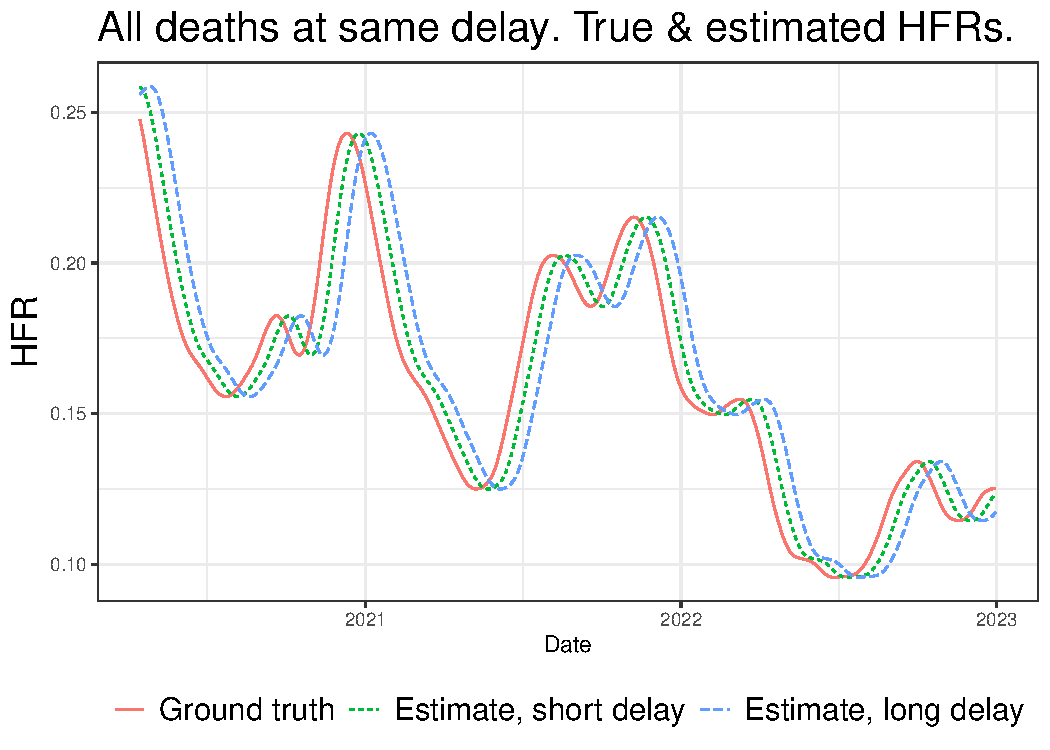
\includegraphics[width=\linewidth]{Figures/Simulated/sim_onehot.pdf} 
         \caption{All deaths after $\ell$ days. HFR ratios equivalent;
         plotting delays of $\ell=14$ and 28 days.} 
         \label{fig:onehot}
     \end{subfigure}
     \hfill
     \begin{subfigure}[b]{0.495\linewidth}
         \centering
         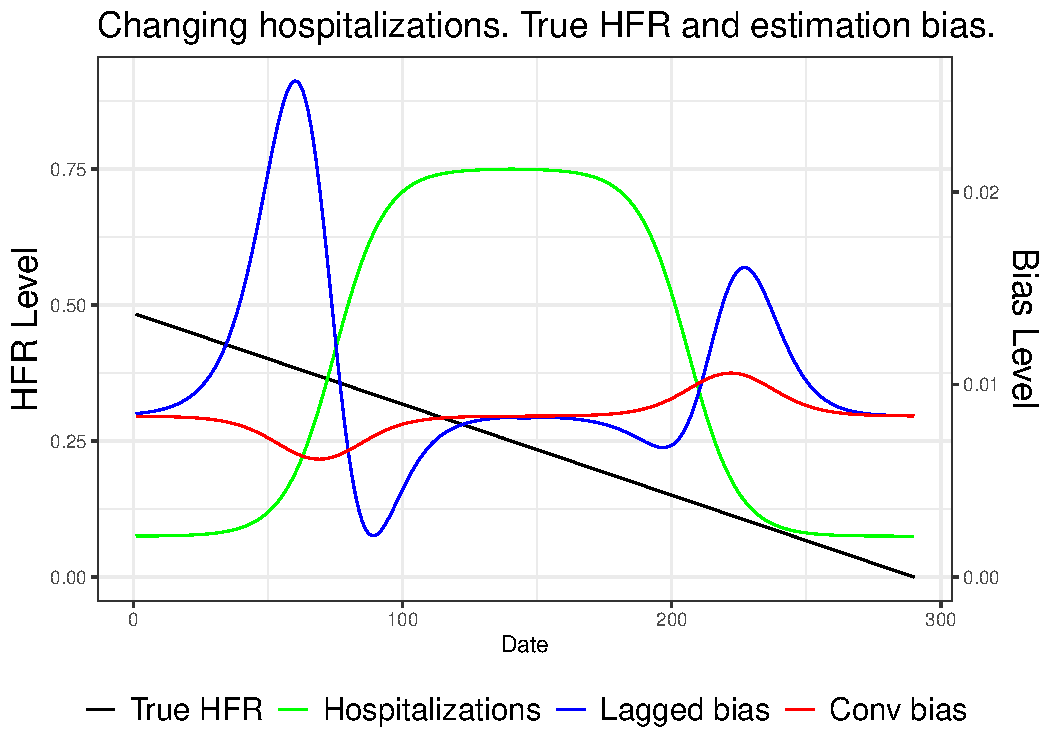
\includegraphics[width=\linewidth]{Figures/Simulated/sim_chging_primary.pdf} 
         \caption{Changing primary incidence. Plotting bias of lagged and
         convolutional ratios.} 
         \label{fig:chging_primary}
     \end{subfigure}
        \caption{Toy examples of biased severity rates.} 
        \label{fig:bias_ex}
\end{figure}


Figure \ref{fig:onehot} displays the results on the NHCS HFRs.
In general, severity rates will be less similar to the present value $p_t$ as we go further back in time. The bias $p_{t-\ell}-p_t$ tends to be larger when $\ell=28$ versus $\ell=14$. This supports the overarching idea
that estimates with heavier-tailed delay distributions tend to have more bias.          

Now to elucidate the relationship between primary incidence and bias, let us 
consider a delay distribution $\pi$ which places half its mass at lag 0, and the
other half at lag $q$. Then the well-specified bias has magnitude:
\[
\big| \bias(\hat{p}_t^{\pi}) \big| = \frac{\frac{1}{2} \big| X_t(p_t-p_t) +
  X_{t-q}(p_{t-q}-p_t) \big|} {\frac{1}{2}(X_t+X_{t-q})} = \frac{|p_{t-q}-p_t|}
{1 + X_t / X_{t-q}}. 
\]
In other words, the absolute bias is monotonically decreasing in
$X_t / X_{t-q}$, the proportion change in primary incidence. Rising  
primary incidence ($X_t / X_{t-q} > 1)$ yields less bias, while falling 
levels yield more. 

Figure \ref{fig:chging_primary} displays this setting with $q=10$. Rising hospitalizations are
defined as \mbox{$X = \sigma(s)*9000+1000$}, where $\sigma$ is the sigmoid function
and $s$ takes 300 evenly spaced steps from -9 to 7. These quantities are subsequently reflected to express a decline.
The true HFRs fall from
0.5 to 0 over the same number of even steps. 
Accordingly, the absolute bias of the convolutional ratio is $c_q\frac{X_{t-q}}{X_{t-q}+X_t}$, where $c_q\approx 0.0167$. Shown in red, it dips as hospitalizations rise, and rises as they fall.  

The figure also plots with lagged ratio with $\ell=\frac{d}{2}$, the mean of
the delay distribution. When daily hospitalizations are close to constant, the
two estimators converge towards the same ratio. During periods of change,
however, the lagged estimator has different bias. It first moves upwards ---
the opposite direction as the convolutional bias --- with far greater
magnitude. This can be explained by the ratio $A_t^\ell =
\frac{X_{t-2\ell}+X_t}{2X_{t-\ell}}$ from Proposition 2. As
hospitalizations begin to steeply rise, $X_{t-2\ell}$ and $X_{t-\ell}$ are
similar, but $X_t > X_{t-\ell}$. Hence, $A_t^\ell>1$, contributing positive
bias to both the oracle and misspecification terms. As hospitalizations level
out near the top, $A_t^\ell < 1$, hence the bias falling lower. The opposite
pattern occurs as hospitalizations fall.  

% Since the convolutional ratio uses the true delay distribution, it has oracle
% bias in Proposition 2. The lagged ratio has lag at the mean
% of the delay distribution, $\ell=\frac{d}{2}$. Its behavior can be explained
% by the ratio $A_t^\ell = \frac{X_{t-2\ell}+X_t}{2X_{t-\ell}}$. As
% hospitalizations begin to steeply rise, $X_{t-2\ell}$ and $X_{t-\ell}$ are
% similar, but $X_t > X_{t-\ell}$. Therefore $A_t^\ell>1$, inflating the
% positive oracle bias term and adding misspecification bias. As
% hospitalizations level out near the top, $A_t^\ell < 1$, hence the bias
% falling lower. The opposite pattern occurs as hospitalizations fall. 

\section{Alternative data sources}
\label{apx:alternatives}

\subsection{Retrospective deaths}
\label{apx:NCHS_deaths}

JHU aggregated daily deaths in real time, aligned by the date they were
reported. In contrast, the National Center for Health Statistics (NCHS) provided
weekly totals of deaths aligned by occurrence, which were not available in real  
time. Intuitively, the delay which relates hospitalization to death occurrence
should have a lighter tail in comparison to that relating hospitalization to
death report. Therefore, since that heavier-tailed delays generally introduce
greater bias, we would expect the ratio estimates computed from JHU deaths to
have greater bias than those from NCHS deaths. Figure \ref{fig:jhu_vs_nchs}
shows that this is indeed the case. NCHS data, which was only available in
retrospect, leads to lagged HFR estimates with substantially less bias.    

\begin{figure}[h]
\centering
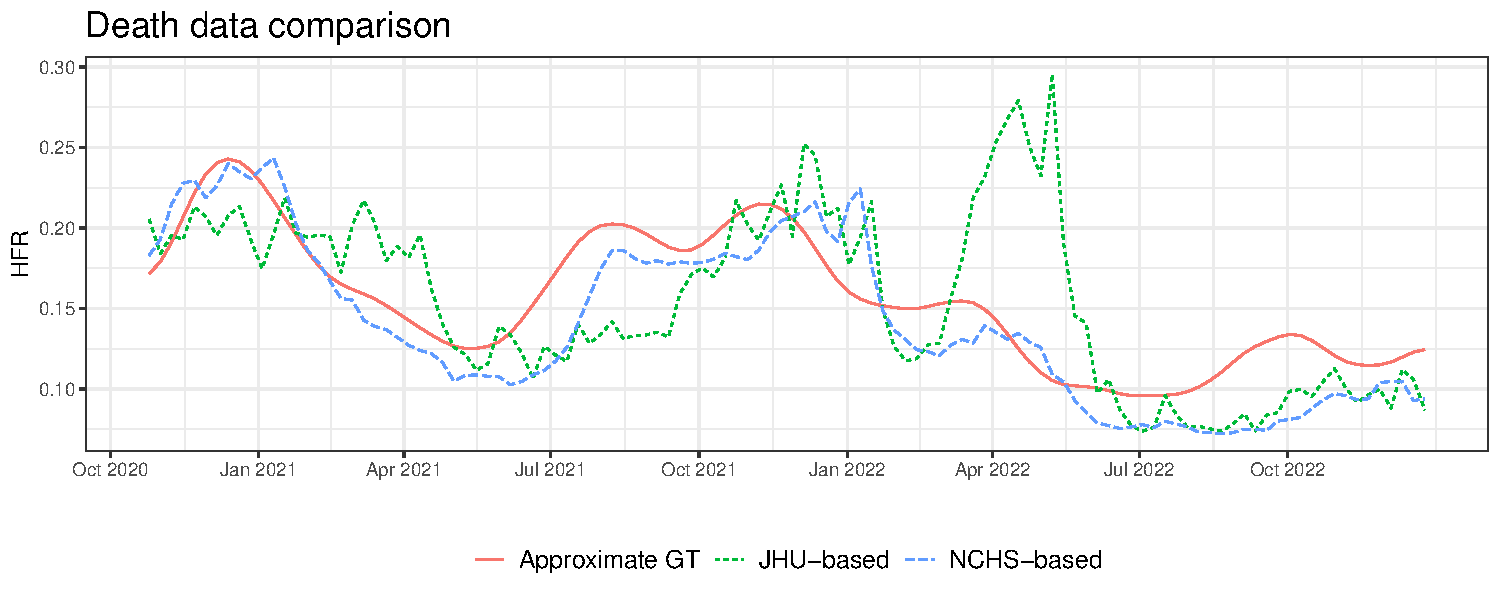
\includegraphics[width=\linewidth]{Figures/Real/jhu_vs_nchs.pdf}
\caption{Comparing lagged ratios based on data from JHU versus NCHS.}
\label{fig:jhu_vs_nchs}
\end{figure}

\subsection{Alternative ground truth}
\label{apx:alt_gt}

\begin{figure}[b!]
\centering
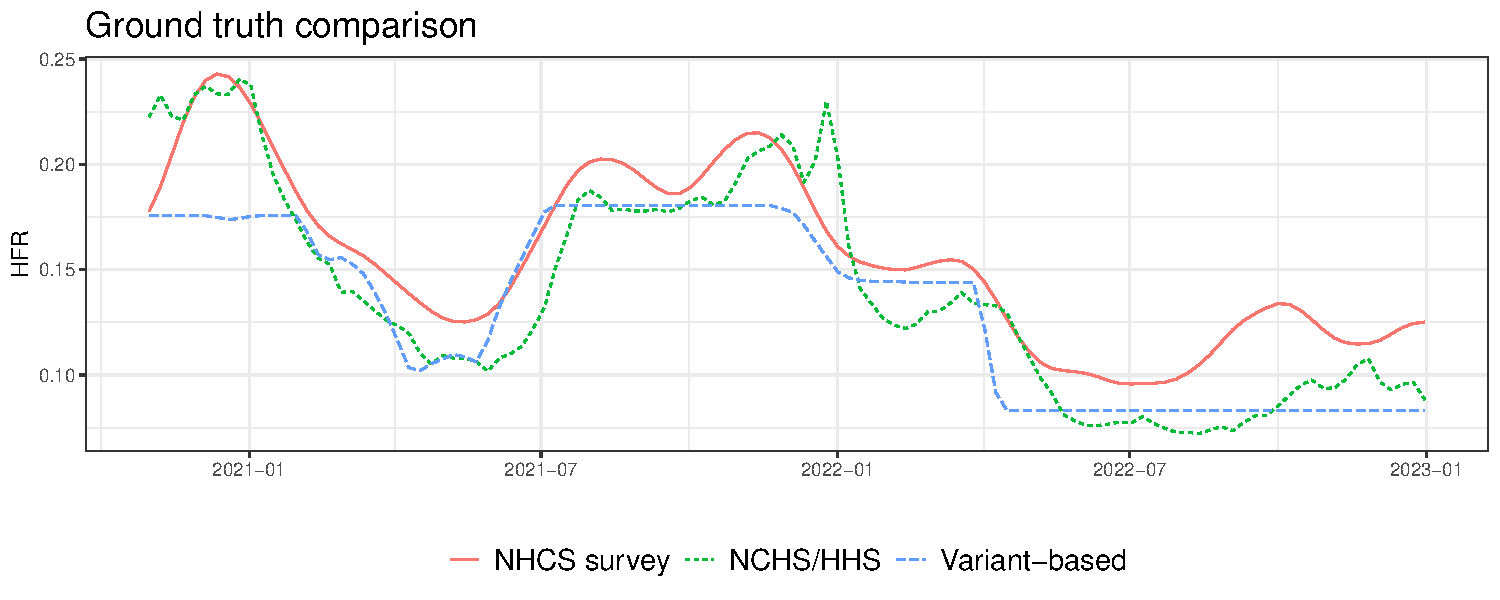
\includegraphics[width=\linewidth]{Figures/Real/ApproxGT.pdf}
\caption{Comparing methods for approximating ground truth HFR.}
\label{fig:approxGT}
\end{figure}

We consider two alternative approaches to approximate the ground truth HFR
curve, over the COVID-19 pandemic. The first is simply to use the lagged ratio
based on NCHS data. As discussed above, this benefits from a lighter-tailed
delay distribution than JHU data. Further, as we are looking to approximate
ground truth in retrospect, we modify this estimator to be forward-looking:
\smash{$\hat{p}_t^\ell = Y_{t+\ell} / X_t$}. The second approach we consider is
to compute a single HFR by dividing total deaths by total hospitalizations in
each major variant period,  
% during the period where it accounted for over 50\% of activate cases 
and then create a smooth curve by mixing these per-variant HFRs by estimates
of the proportion of variants in circulation, obtained from CoVariants.org. We only consider the four largest variants: the original
strain, Alpha, Delta, and Omicron. However, because Omicron began with an
enormous surge that quickly subsided, we split it into early and late periods.
%following \citep{adjei2022mortality}

Figure \ref{fig:approxGT} displays these two alternative ground truth curves,
alongside that obtained from NHCS. They have nontrivial differences in
magnitude, but reassuringly, the three curves move more or less in
conjunction. The retrospective NCHS ratio is still subject to statistical bias
similar to equation (7); the variant-based HFR curve is flatter, as it 
does not account for other sources of potential variability in the underlying
severity rate.   

\section{Robustness checks}
\label{apx:robustness}

\subsection{Real-time versus finalized data}

Recall, the results in Section 3.1 use hospitalization and
death counts available in real time. To investigate the sensitivity of our
findings, we recompute the lagged and convolutional ratios, this time using
finalized counts. Figure \ref{fig:rt_and_final} shows the real-time and
finalized estimates track one another very closely. Therefore, the observed bias
in Figure 3 cannot be attributed to real-time
reporting quirks.  

% The one period where the curves are significantly different from one another
% is in March 2022. While the HFRs from finalized counts steadily rise, the
% real-time estimates sharply fall then immediately bounce back. This sudden
% drop is due to a brief period in which reported death counts were suddenly too
% low (Fig. \ref{fig:source}. This is corrected in the finalized counts, hence
% their smooth HFRs. Removing this artifact further reinforces the bias trends
% described in Section~\ref{sec:wellspecified}. 

\begin{figure}[htb]
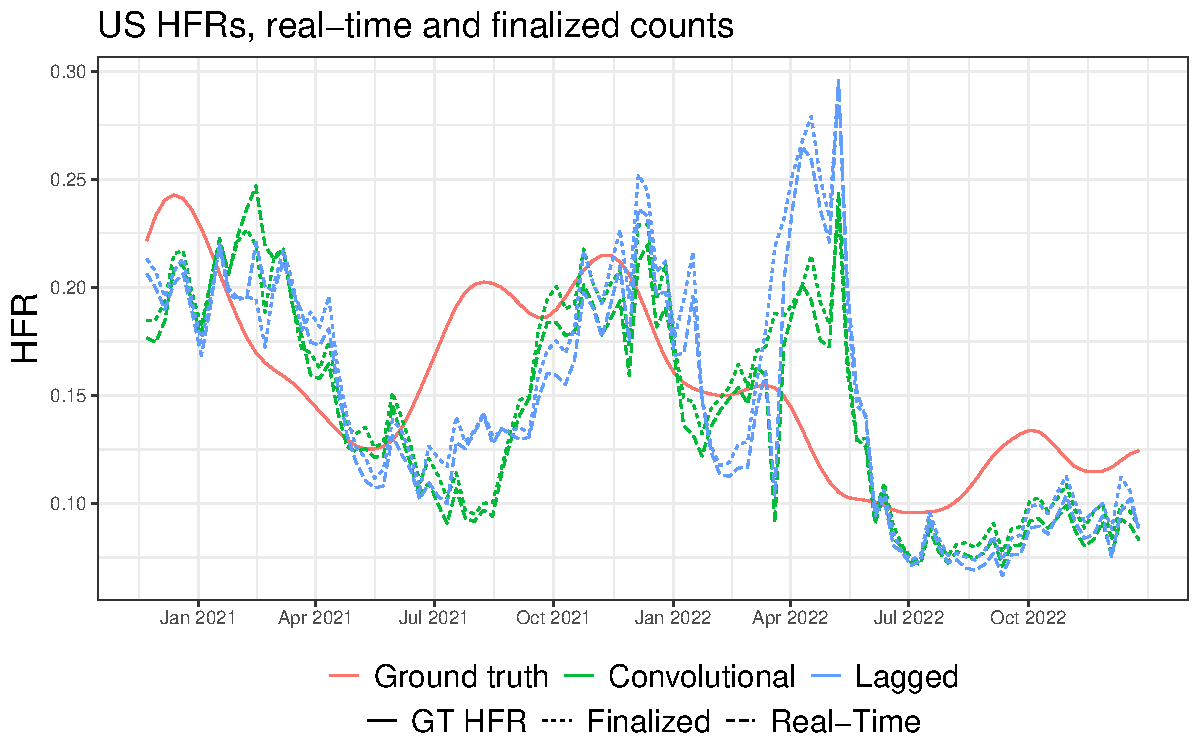
\includegraphics[width=\linewidth]{Figures/Real/US_ests_realtime_both.pdf}
%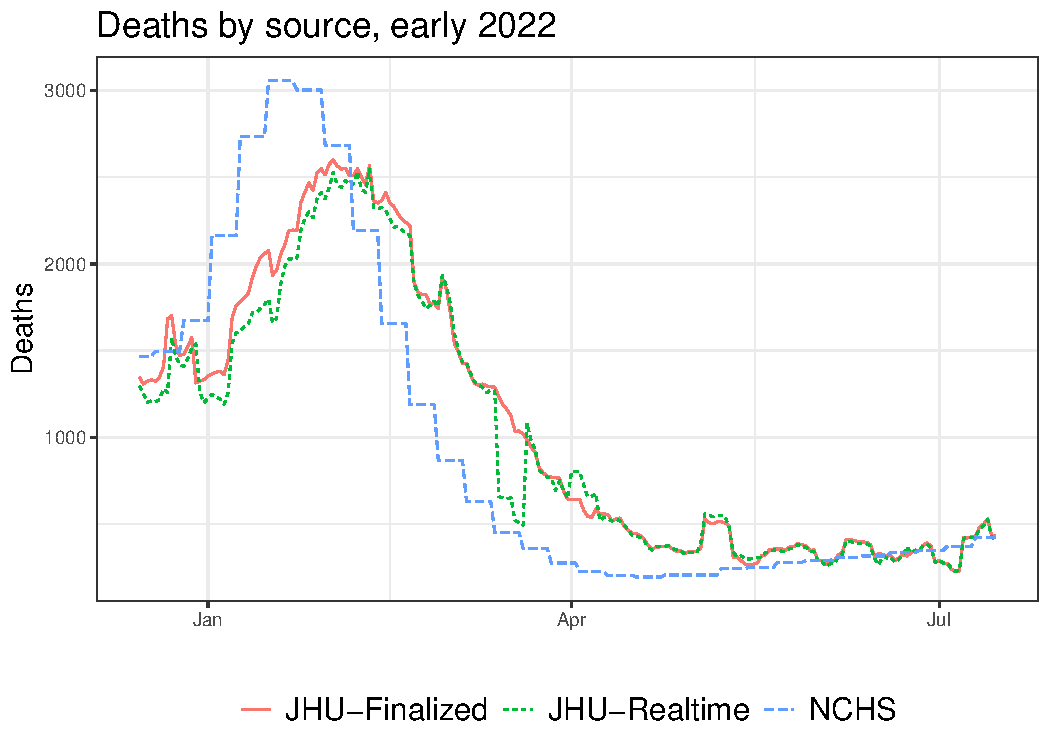
\includegraphics[width=\linewidth]{Figures/Real/death_curves.pdf}
\caption{Comparing estimates based on real-time versus finalized counts.}    
\label{fig:rt_and_final}
\end{figure}

\subsection{Hyperparameters}

We evaluate the robustness of our findings against choices of hyperparameters.
% (All results henceforth are with the finalized version of JHU deaths.) 
First, we analyze smoothed versions of the ratio estimators, where we smooth the 
numerator and denominator separately:
\begin{align*}
\hat{p}_t^{\ell,w} &= \frac{\sum_{s=t-w+1}^t Y_s}
{\sum_{s=t-w+1}^t X_{s-\ell}}, \\ 
\hat{p}_t^{\gamma,w} &= \frac{\sum_{s=t-w+1}^t Y_s}
{\sum_{s=t-w+1}^t \sum_{k=0}^d X_{s-\ell-k}\gamma_k}.
\end{align*} 
Figure \ref{fig:window} shows the results for varying window lengths $w >
0$. The results are very similar, indicating the bias does not disappear when
smoothing over a longer history.  

\begin{figure}[h!]
\centering
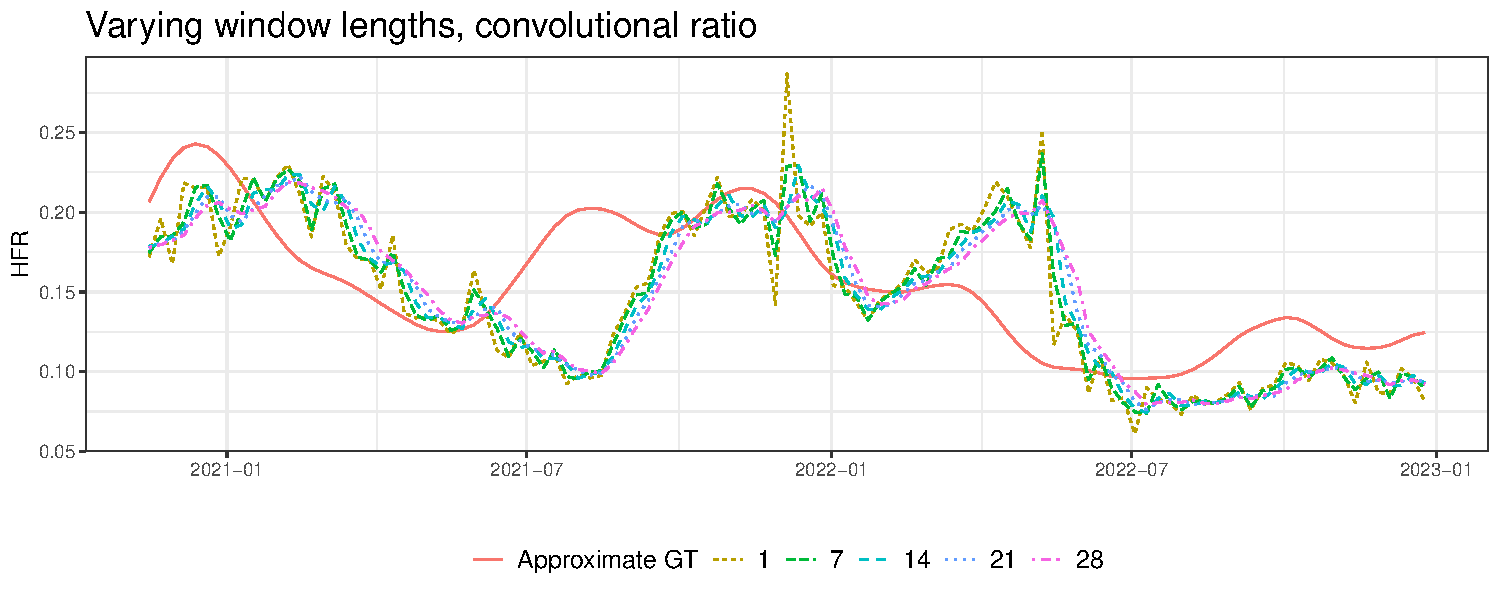
\includegraphics[width=.95\linewidth]{Figures/Real/window_size_conv.pdf}
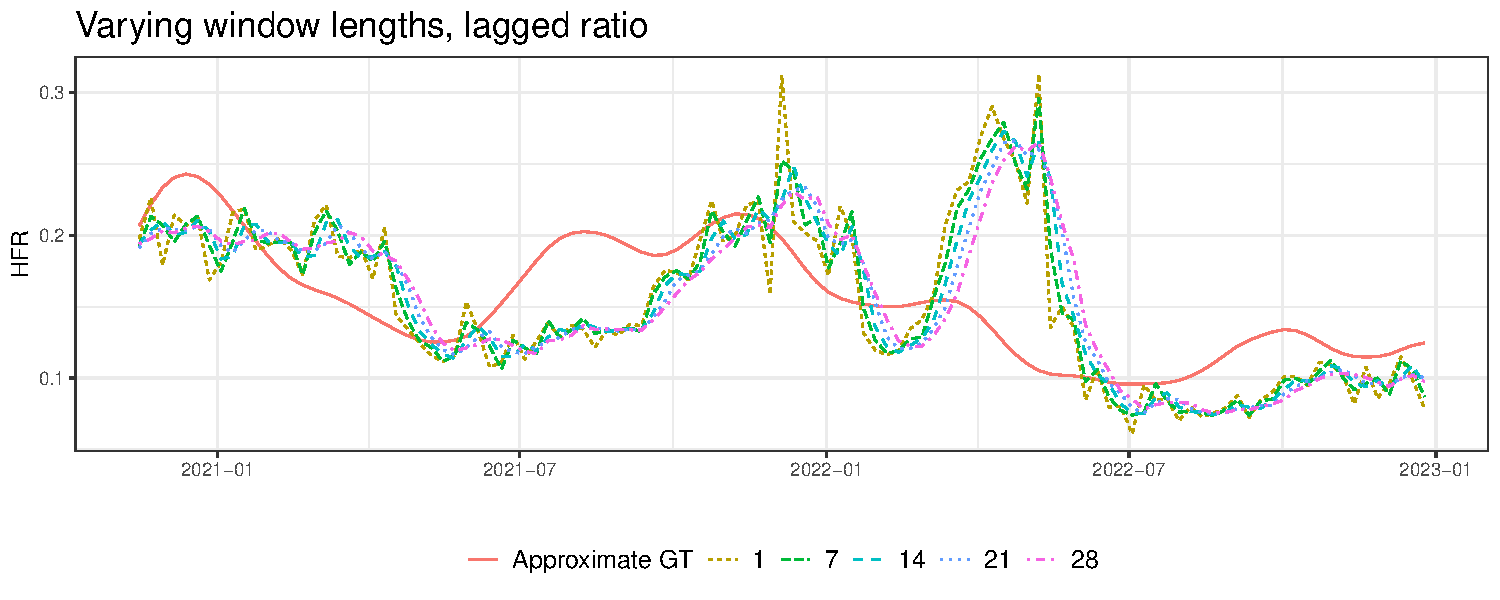
\includegraphics[width=.95\linewidth]{Figures/Real/window_size_lagg.pdf}
\caption{Comparing different choices of window length in post-smoothing.}
\label{fig:window}
\end{figure}

We next examine the time-to-death hyperparameters: The lag for the lagged ratio
and delay distribution for the convolutional ratio. Figure \ref{fig:lag}
displays lagged HFR estimates where the lag $\ell$ ranges from 2 to 5
weeks. Unlike the window size, changing this parameter leads to notably
different behavior. Some choices of lag are better than others; a 28-day lag,
for example, falls appropriately in winter 2021, and rises less slowly during
Delta. However, all are biased to varying degrees, most notably the huge
spurious surge in spring 2022.

\begin{figure}[p]
\centering
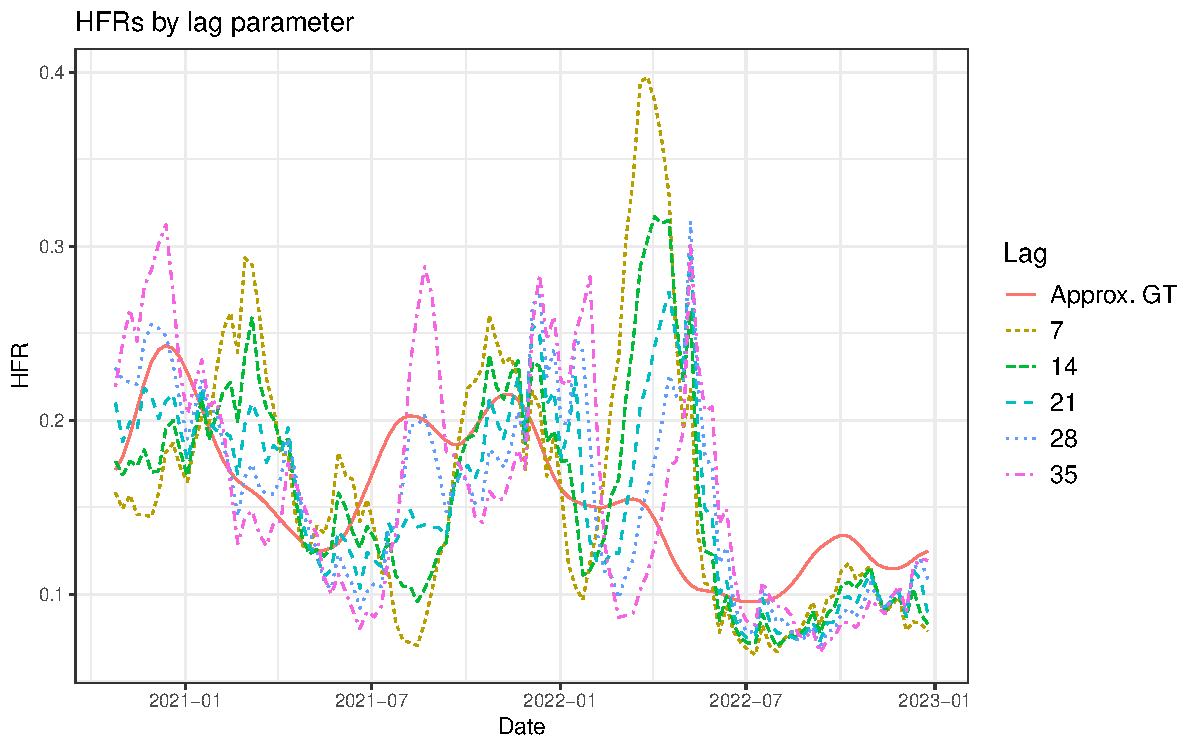
\includegraphics[width=\linewidth]{Figures/Real/hfrs_by_lag.pdf}
\caption{Comparing different choices of lag parameter in the lagged ratio.}
\label{fig:lag}

\bigskip
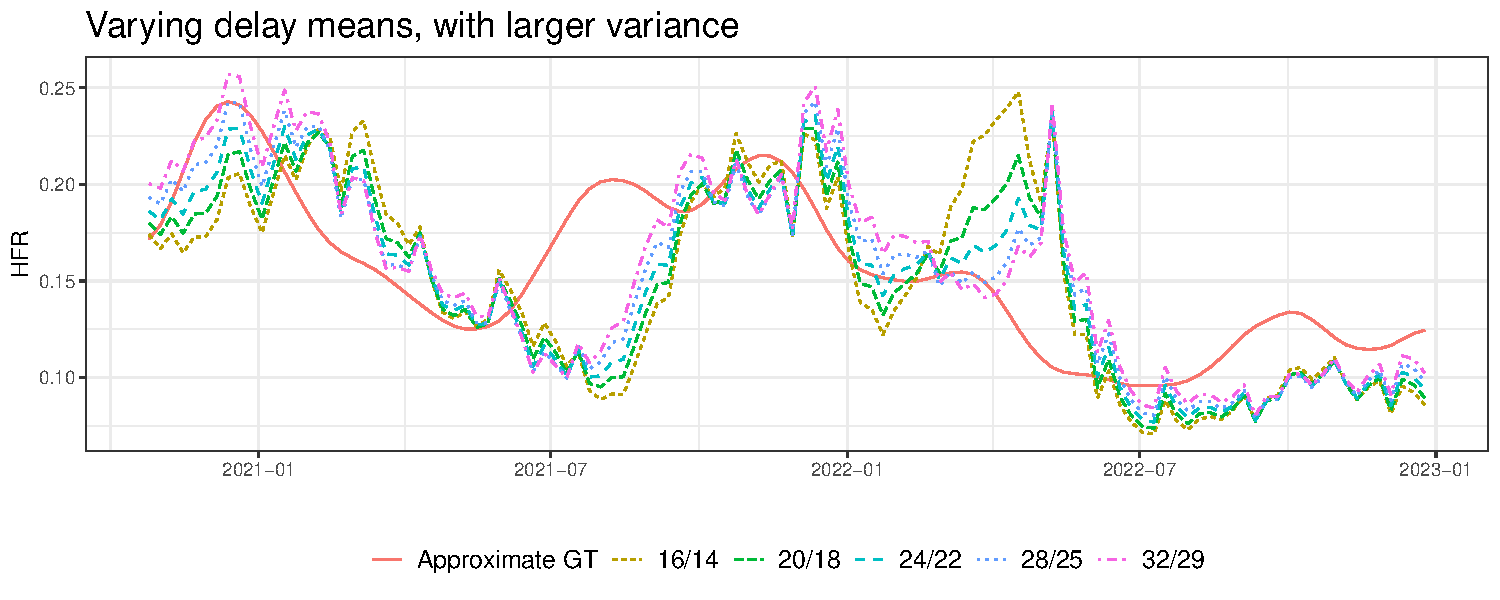
\includegraphics[width=\linewidth]{Figures/Real/hfrs_by_delay1.pdf}
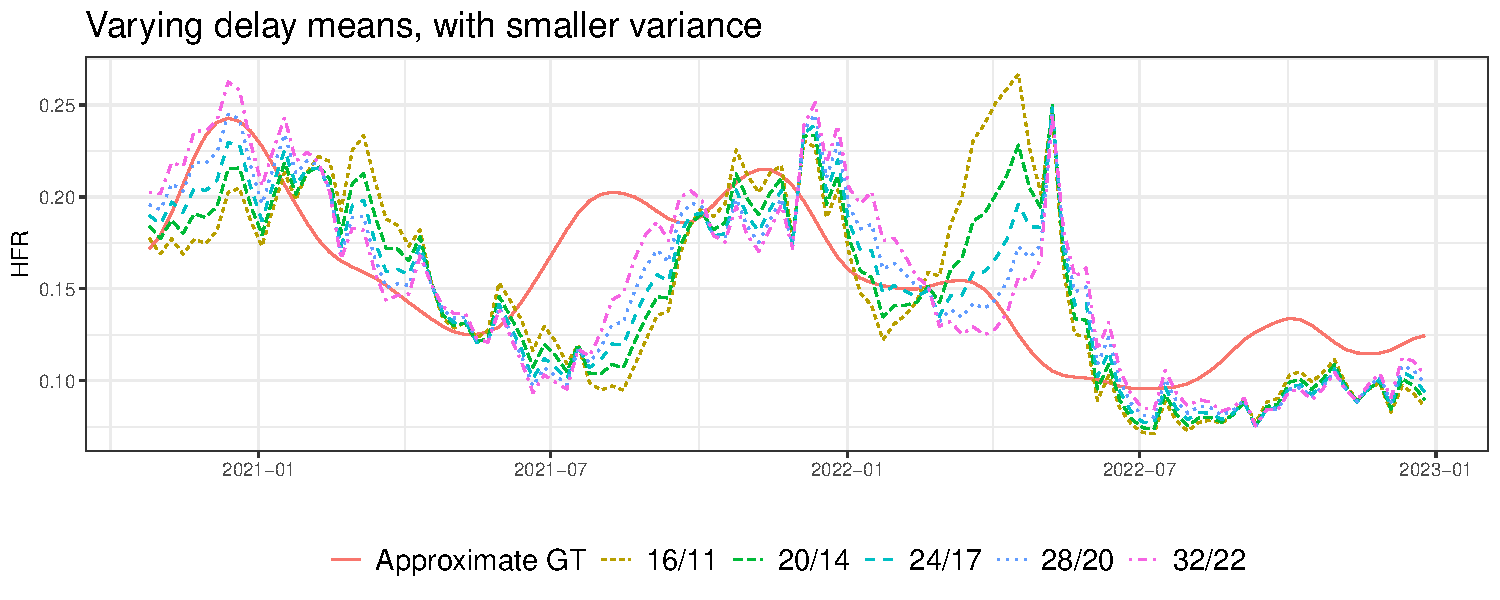
\includegraphics[width=\linewidth]{Figures/Real/hfrs_by_delay2.pdf}
\caption{Comparing different choices of delay distributions in the convolutional
  ratio. The top panel shows gamma distributions whose standard deviation is 0.9
  times the mean, versus 0.7 times the mean the bottom panel. The legend labels
  reflect the mean/standard deviation.}  
\label{fig:delays}
\end{figure}

Figure \ref{fig:delays} compares the performance of the convolutional ratio
across different choices of delay $\gamma$; we kept the discrete
gamma shape for each, but varied the mean and standard deviation. We
investigated a standard deviation equal to 90\% of the mean, and also a more
compact delay with standard deviation equal to 70\% of the mean. All
resulting HFR estimates are significantly biased. Regardless of delay
distribution, the ratios are negatively biased during the onset of Delta, and
surge after the peak of Omicron. This indicates the bulk of the error is
fundamental to the estimator, and cannot be attributed to model
misspecification.     

% Comparing to the approximate ground truth HFRs from NHCS, performance improved 
% slightly with a longer delay distribution than the purported mean of 20 
% days. Its mean absolute error was 0.031, whereas the delay distribution with 
% mean 28 and standard deviation 25 had a MAE of 0.27. Nevertheless, this 
% difference is relatively small, with the alternative delay distribution still 
% showing similar bias.  

\subsection{State-level results}

We repeat our analysis the six large US states, finding similar trends. The NHCS
survey was conducted on a subset of hospitals meant to represent the US at
large, so for the state-level approximate ground truth, we therefore use the
forward-looking lagged ratio computed using NCHS deaths, as discussed above.
Figure \ref{fig:state-level} compares this rough ground truth to the real-time 
convolutional and lagged ratios. For each state, we select the lag for the
approximate ground truth curve to maximize cross-correlation between
hospitalizations and NCHS deaths, and the lag in the real-time lagged ratio to
maximize cross-correlation between hospitalizations and JHU deaths. We then use
a discrete gamma distribution with mean equal to the latter lag, and standard
deviation 90\% of its mean, for the convolutional ratio.

\begin{figure}[htbp]
\centering
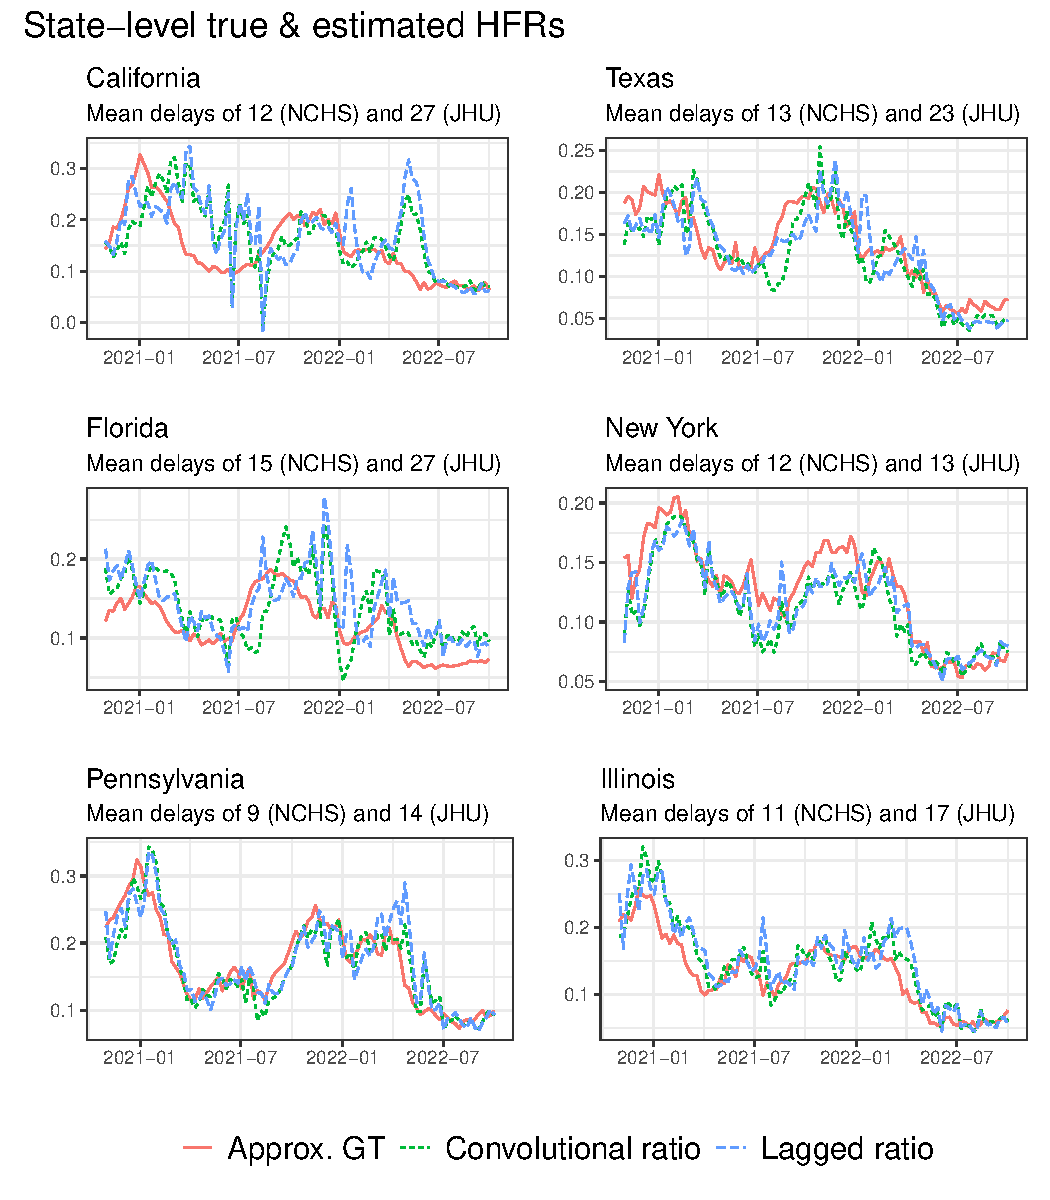
\includegraphics[width=\linewidth]{Figures/Real/state_level_hfrs.pdf}
\caption{Comparing ratio estimates for individual US states.} 
\label{fig:state-level}
 \end{figure}

Several states display similar biases to the US as whole (Figure
3). Estimates in California, Texas, and Florida are 
all slow to detect the uptick in HFR during Delta; they also spike during
Omicron in California, and to a lesser extent Florida. Note these states are the
ones with the largest cross-correlation optimal lags, an estimate of the average 
time-to-death. In contrast, New York, Pennsylvania, and Illinois have mean delays
of at most 17. Their HFR estimates are still biased, but overall less so. This
once again emphasizes the role of the delay in bias. The takeaway: fatality
ratios are generally less trustworthy in states that take longer to report
deaths.         


\end{document}